\chapter*{Preface.}

{\scshape The aim} of this paper is to provide a self-contained exposition of the proof of the Conway-Schneeberger Fifteen Theorem provided by Manjul Bhargava in \cite{bhargava2000conway}. The theorem states that for a positive-definite integer-valued quadratic form to represent all positive integers, it is necessary and sufficient that it represent all positive integers up to \(15\). The original proof by Conway was never published, although in 1995, William Schneeberger has provided a sketch of the proof in his Ph.D. thesis. \cite{schneeberger1997arithmetic} The proof we examine here was provided by Bhargava in 2000, relying heavily on the theory of genera and of lattices; Bhargava was later to generalize this in what would later be known as the \(290\) theorem. \cite{bhargava2005universal} For this and his other contributions to number theory, in particular to the geometry of numbers, Bhargava was awarded the Fields Medal in 2014. \cite{bhargava2014fields}

While the author has endeavoured to make this exposition as self-contained as possible, some elementary results have been omitted and throughout the paper, the reader will be assumed to have a basic understanding of number theory, linear algebra, and abstract algebra, on the level of the introductory graduate courses on those subjects in De La Salle University. 

Chapter \ref{chap:quadratic-forms} provides an introduction of the theory of quadratic forms over a field \(\field\) of characteristic not equal to \(2\) and the equivalent notions of Gram matrices and symmetric bilinear forms, following the treatment in \cite{lam1973quadratic}. The main results in the chapter include the equivalence of quadratic forms to a diagonal form as well as some results specific to the number theoretic treatment of rational and integral quadratic forms from \cite{cassels2008rational} and \cite{jones1950arithmetic}. Chapter \ref{chap:local-global-principle} is essentially an exposition of Chapters 2--4 of Serre's \emph{Course in Arithmetic} \cite{serre2012course}. In it, we construct the field \(\Rationals_p\) of \(p\)-adic numbers, develop the theory of quadratic forms in \(\Rationals_p\) and \(\Rationals\), and finally prove the Hasse-Minkowski theorem. We then explore some consequences of this theorem and its applications to number theory. In Chapter \ref{chap:integral-quadratic-forms} we introduce the language of lattices to study quadratic forms over the the rings \(\Integers\) and \(\Integers_p\) in order to investigate how, if at all possible, to extend the results of Chapter \ref{chap:local-global-principle} to analogues for principal ideal domains, in particular \(\Integers\). The exposition in this chapter follows closely the treatment in \cite{cassels2008rational,gerstein2008basic,jones1950arithmetic}. Chapter \ref{chap:conway-schneeberger} uses the results of the previous chapters to prove the Conway-Schneeberger Fifteen Theorem using the method of escalating lattices. We follow the original exposition in \cite{bhargava2000conway}, as well as \cite{moon2008universal}. We conclude by quickly reviewing the \(290\) theorem of Bhargava and Hanke \cite{bhargava2005universal}, which generalizes the Fifteen Theorem for integral quadratic forms (in the sense of \S\,\ref{sec:integral-forms-def}).


\begin{figure}
    \centering
    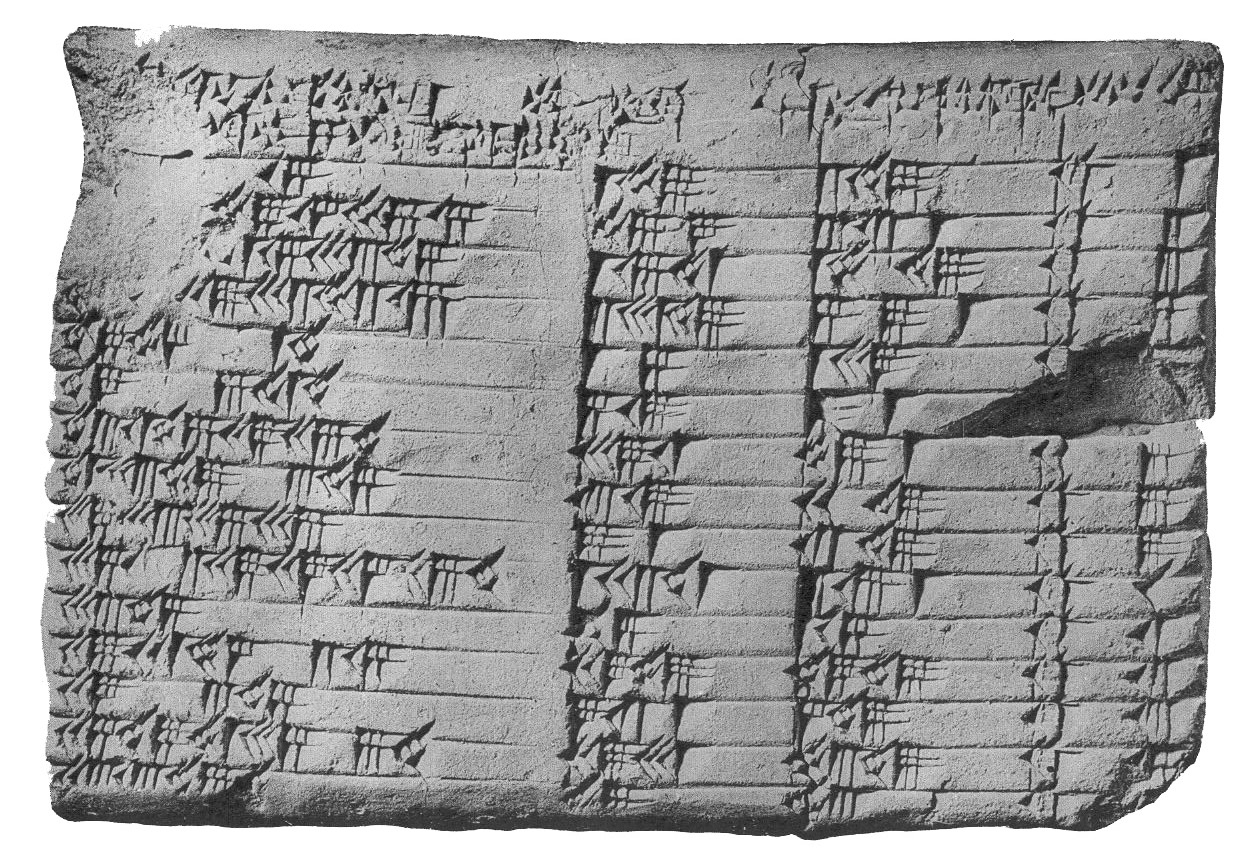
\includegraphics[width=\textwidth]{assets/Plimpton_322.jpg}
    \caption[The Plimpton 322 tablet.]{The Plimpton 322 tablet. Image from Wikimedia Commons.}
    \label{fig:plimpton-322}
\end{figure}

\begin{figure}
    \centering
    \includegraphics[width=0.8\textwidth]{assets/euclid.png}
    \caption[A geometric construction of Pythagorean triples.]{A geometric construction of Pythagorean triples from Euclid's \emph{Elements}. Image from the Greek text prepared by Heiberg. \cite{heiberg1885euclid}}
    \label{fig:pythagorean-triples}
\end{figure}

\section*{A historical note.}


A quadratic form is a homogeneous polynomial of degree two (form, in this case, being a dated term for a homogeneous polynomial). The theory of quadratic forms has a long and rich history, with some of the earliest results dating back to antiquity. For example, integer solutions to the equation
\[
    x^2 + y^2 = z^2 
\]
have been known to the ancient Babylonians,referred to as Pythagorean triples, although the results likely predate the Pythagoreans. A table of fifteen triples have been preserved in a tablet that has come to be labelled as Plimpton 322 (after its provenance) and has been dated to between the 19th and 16th centuries {\lsstylehelp{100}\sc b.c.e.} \cite{robson2002words} Euclid (fl. 300 {\lsstylehelp{100}\sc b.c.e.}), in Book X, Prop.\,29, of his \emph{Elements}, has demonstrated a way of constructing Pythagorean triples geometrically. \cite{euclid1956elements} Following Euclid, the next substantial treatment of quadratic forms (and of classical number theory, in general) was given by Diophantus of Alexandria in his \emph{Arithmetica}, which has served as the prototypical number theory text for much of antiquity and the Middle Ages. \cite{katz2009history} Thus for any pair of integers \(m\) and \(n\) with \(m > n\), the triple
\(
    (2mn, m^2 - n^2, m^2 + n^2)
\)
is a Pythagorean triple. These results has been attested to have developed separately in the Indian and Chinese mathematical traditions as well. \cite{weil1984number}

The work of Diophantus on the theory of numbers continued to be expanded upon both by Islamic mathematicians during the Middle Ages, including in treatises by al-Khwarizmi (fl. 800 {\lsstylehelp{100}\sc c.e.}) and European mathematicians like Vi\`ete, Bachet, and Pacioli during the Renaissance. In the 18th century, Pierre de Fermat and Leonhard Euler have shown that all prime numbers of the form \(4n + 1\) can be represented by a sum of squares.\,\cite{hahn2008quadratic} Later on Fermat and Joseph-Louis Lagrange have expanded this to sums of the form \(x^2 + Ny^2\) for some integer \(N\). Perhaps the most famous result of this period is Lagrange's assertion that every whole number can be expressed as the sum of four squares. Fermat, during this time, has introduced one of the longest-standing open problems in number theory, his ``last theorem'' about how there are no integer solutions to the equation \(x^n + y^n = z^n\) for \(n > 2\). While this problem is not directly related to quadratic forms, it has significantly influenced the development of the theory of numbers in the centuries since, culminating in a solution by Andrew Wiles in 1995. \cite{wiles1995modular}

At the turn of the century, Carl Friedrich Gauss published what was to become the most influential work on number theory, \emph{Disquisitiones Arithmetic\ae}. It is difficult to overstate the effect that Gauss’s \emph{Disquisitiones} has had on the development of the theory of numbers. This work is to cast a long shadow on the work of mathematicians in the the time since its original publication, not least because of the sheer scope of its contents. Two centuries after \emph{Disquisitiones} first appeared, the mathematician John Conway was to remark, for example,
\begin{quote}
    [W]hen Neil Sloane and I wanted to summarize the classification theory of binary forms for one of our books, we found that the only Number Theory textbook in the Cambridge Mathematical Library that handled every case was still the \emph{Disquisitiones}! \cite{conway1999universal} 
\end{quote}
In \emph{Disquisitiones}, Gauss has introduced, among other things, important results in congruence,\,---\,a notion which remains a central concept in modern number theory; much of the number theoretic notation still used to this day can be traced back to this book by Gauss, in particular writing
\[
    a \equiv b \quad (\text{mod. } m)
\]
to indicate that \(a\) and \(b\) are ``congruent'' under the  ``modulus'' \(m\). (The dot after the original abbreviation was soon to disappear.) More than half of the six-hundred-odd pages of \emph{Disquisitiones} is devoted to the theory of quadratic forms and quadratic reciprocity, which Gauss has exhaustively studied. 

Throughout the nineteenth century, work on quadratic forms continued, building on the foundations laid by Gauss. The reduction and classification theories in the \emph{Disquisitiones} was completed by James Joseph Sylvester (in his famous ``law of inertia'') over the real numbers. The French mathematician Charles Hermite has provided useful bounds for reducing quadratic forms over \(\Integers\) using the concept of the minimum of a positive-definite quadratic form. \cite{gerstein2008basic} (We shall review some of these results in Chapter \ref{chap:quadratic-forms}.) Towards the end of the nineteenth century, Hermann Minkowski introduced the ``local-global'' principle for the classification of quadratic forms. The introduction by Kurt Hensel in 1897 of \(p\)-adic numbers, and the work on valuation theory by his student Helmut Hasse, has allowed for the extension of the local-global principle to a more general number-theoretic setting. \cite{gerstein2008basic,hensel1913zahlentheorie,hasse1922uber} We shall develop the results from Minkowski, Hensel, and Hasse as they apply to quadratic forms in Chapter \,\ref{chap:local-global-principle}.